\documentclass[12pt,a4paper]{article}
\usepackage[utf8]{inputenc}
\usepackage[french]{babel}
\usepackage{hyperref}
\usepackage{amsmath, amssymb}
\usepackage{graphicx} % Nécessaire pour \includegraphics
\usepackage[T1]{fontenc}
\usepackage[none]{hyphenat} % Désactive la césure des mots

\title{Résumé et Analyse de l’algorithme cyclique pour l’estimation du maximum de vraisemblance utilisant le complément de Schur}
\author{KABLAM EDJABROU ULRICH BLANCHARD}
\date{25 Mai 2025} % Vous pouvez mettre \today pour la date actuelle

\begin{document}
	
	\maketitle
	
	\tableofcontents
	
	\newpage
	
	\section{Introduction}
	L'estimation paramétrique à partir de données observées est une démarche centrale en statistique et en modélisation, trouvant des applications dans une multitude de disciplines scientifiques. La méthode du maximum de vraisemblance (MLE) \cite{ref1, ref2, ref3} s'impose comme une technique d'optimisation numérique de référence, permettant d'identifier les paramètres d'un modèle probabiliste qui maximisent la plausibilité des observations. Cette maximisation, qu'elle soit contrainte ou non, s'opère souvent sur le logarithme de la fonction de vraisemblance pour des raisons pratiques, notamment dans la modélisation de répartitions catégorielles via la loi multinomiale. Si, dans des cas simples, l'estimation des probabilités de classe découle directement des fréquences observées, la réalité des applications introduit fréquemment une dépendance à des paramètres auxiliaires eux-mêmes soumis à des contraintes.
	
	La présence de ces paramètres auxiliaires contraints complexifie significativement l'estimation du maximum de vraisemblance. Les méthodes d'optimisation traditionnelles, telles que les algorithmes basés sur la méthode de Newton, se heurtent alors à des défis computationnels majeurs, en particulier lorsque le nombre de paramètres est élevé ou que les modèles présentent des structures de dépendance complexes. Le calcul et l'inversion répétés de matrices Hessiennes de grande dimension deviennent alors un goulot d'étranglement, limitant l'applicabilité et l'efficacité de ces approches classiques dans de nombreux contextes pratiques.
	
	Face à ces limitations, le présent document se propose d'analyser une alternative prometteuse : un algorithme cyclique pour l'estimation du maximum de vraisemblance sous contraintes, développé par N'Guessan et Geraldo, qui tire parti des propriétés du complément de Schur. L'hypothèse sous-jacente est que cette approche peut significativement simplifier le processus d'optimisation, notamment en évitant les calculs matriciels lourds, et ainsi offrir une meilleure efficacité computationnelle par rapport aux méthodes établies. Pour vérifier cette hypothèse, nous examinerons en détail les fondements théoriques de cet algorithme, son fonctionnement étape par étape, et nous évaluerons ses performances, en particulier dans le contexte d'applications concrètes telles que l'analyse de données en sécurité routière.
	
	\section{Résumé de l’article} % Correspond à "## Résumé"
	Voici un résumé détaillé du document "A cyclic algorithm for maximum likelihood estimation using Schur complement" d’Assi N’Guessan et Issa Cherif Geraldo, avec explications des notions principales, références citées, et des liens vers les concepts pour approfondir.
	
	\subsection*{Résumé du document original} % Pour ne pas numéroter ce sous-titre
	Ce travail propose un nouvel algorithme cyclique pour l’estimation du maximum de vraisemblance sous contraintes, utilisant le complément de Schur pour résoudre le problème d’optimisation. L’algorithme est conçu pour des situations où les paramètres inconnus peuvent être séparés en deux groupes, ce qui permet une résolution alternée (par blocs) et explicite des équations d’estimation, évitant ainsi le calcul coûteux de la matrice Hessienne habituellement requis dans les méthodes classiques comme Newton-Raphson ou BFGS.
	
	Les auteurs démontrent que leur approche est plus rapide que les méthodes traditionnelles, notamment dans des cas pratiques de grande dimension ou de contraintes complexes, et l’appliquent à l’évaluation de politiques de sécurité routière à travers des simulations numériques.
	
	\section{Notions principales} % Correspond à "## Notions principales détaillées"
	
	\subsection{Matrice symétrique définie positive}
	Soit $A=(a_{ij})_{1\leq i,j \leq n}$ une matrice réelle. A est dite:\\
	1.  Symétrique si: \\
	$A = A^T$. Autrement dit pour tous les indices entiers $i, j : a_{i,j} = a_{j,i}.$
	
	2. Définie positive:\\
	Pour tout vecteur non nul X $\in \mathbb{R}^n$, on a $X^TAX > 0.$\\ 
	\url{https://www.bibmath.net/dico/index.php?action=affiche&quoi=./m/matsympos.html}
	
	\subsection{Maximum de vraisemblance (MLE)}
	Méthode statistique pour estimer les paramètres d’un modèle probabiliste en maximisant la probabilité d’observer les données recueillies.
	
	Généralement, on maximise la log-vraisemblance sous contraintes (par exemple, la somme des probabilités de classes égale à 1).
	
	Voir la définition détaillée de la méthode du maximum de vraisemblance : \url{https://fr.wikipedia.org/wiki/Maximum_de_vraisemblance}
	
	\subsection{Complément de Schur}
	Outil d’algèbre linéaire permettant de simplifier l’inversion de matrices partitionnées, crucial ici pour obtenir une solution explicite sans calculer la Hessienne entière.
	
	En savoir plus sur le complément de Schur : \url{https://www.cis.upenn.edu/~jean/schur-comp.pdf} \\
	Vidéo sur le Schur Complement : \url{https://www.youtube.com/watch?v=3d_-klrMZLw&t=19s}
	
	\subsection{Optimisation sous contraintes}
	Problème où l’on maximise (ou minimise) une fonction objectif sous des contraintes d’égalité ou d’inégalité sur les paramètres.
	
	Ici, les contraintes sont linéaires (par exemple, somme des probabilités égale à 1) et de bornes (chaque probabilité entre 0 et 1).
	
	\subsection{Méthodes classiques comparées}
	\begin{itemize}
		\item \textbf{Newton-Raphson :} nécessite le calcul de la Hessienne, coûteux en grande dimension. \\
		Lien : \url{https://fr.wikipedia.org/wiki/M%C3%A9thode_de_Newton}
		\item \textbf{Quasi-Newton (BFGS) :} approche la Hessienne via le gradient, plus efficace mais encore coûteuse. \\
		Lien : \url{https://en.wikipedia.org/wiki/Broyden%E2%80%93Fletcher%E2%80%93Goldfarb%E2%80%93Shanno_algorithm}
		\item \textbf{Nelder-Mead :} méthode sans dérivées, adaptée à certains cas mais moins performante en présence de contraintes complexes. \\
		Lien : \url{https://fr.wikipedia.org/wiki/M%C3%A9thode_de_Nelder-Mead}
	\end{itemize}
	
	% La section suivante "Description de l'algorithme cyclique"
	% reprend les points 5 et 7 de vos informations.
	
	\section{Description de l’algorithme cyclique}
	\subsection{Principe de l'algorithme cyclique proposé} % Correspond au point 5
	L'algorithme partitionne les paramètres en deux groupes, alternant leur estimation.
	Il utilise le complément de Schur pour obtenir la solution du sous-système linéaire à chaque étape, sans recourir à la Hessienne.
	Il converge plus rapidement dans les simulations, notamment pour des données de type multinomiale et des applications en sécurité routière.
	
	\subsection{Fonctionnement détaillé} % Correspond au point 7
	L'algorithme cyclique proposé par N’Guessan et Geraldo fonctionne de la manière suivante :
	\begin{itemize}
		\item \textbf{Décomposition :} Les paramètres inconnus du modèle de maximum de vraisemblance sont divisés en (au moins) deux groupes (blocs).
		\item \textbf{Cycle d'estimation :}
		\begin{itemize}
			\item \textit{Étape A :} Estimer le premier groupe de paramètres en considérant le second groupe comme fixe (en utilisant leurs valeurs actuelles). Le complément de Schur est utilisé ici pour simplifier cette étape.
			\item \textit{Étape B :} Estimer le second groupe de paramètres en considérant le premier groupe comme fixe (en utilisant les valeurs nouvellement mises à jour de l'étape A).
		\end{itemize}
		\item \textbf{Répétition :} Répéter les étapes A et B (le cycle) jusqu'à ce que les estimations des paramètres convergent (ne changent plus significativement).
	\end{itemize}
	
	\subsection{Autres notions liées à l'algorithme}
	
	\subsubsection{Loi ou distribution multinomiale (cas particulier: loi binomiale)} % Correspond au point 8
	Vidéo d'explication (Anglais) : \url{https://www.youtube.com/watch?v=BZxCIkSkMgo}
	\begin{figure}[h!] % h! pour forcer la position ici, ajustez si besoin (htbp)
		\centering
		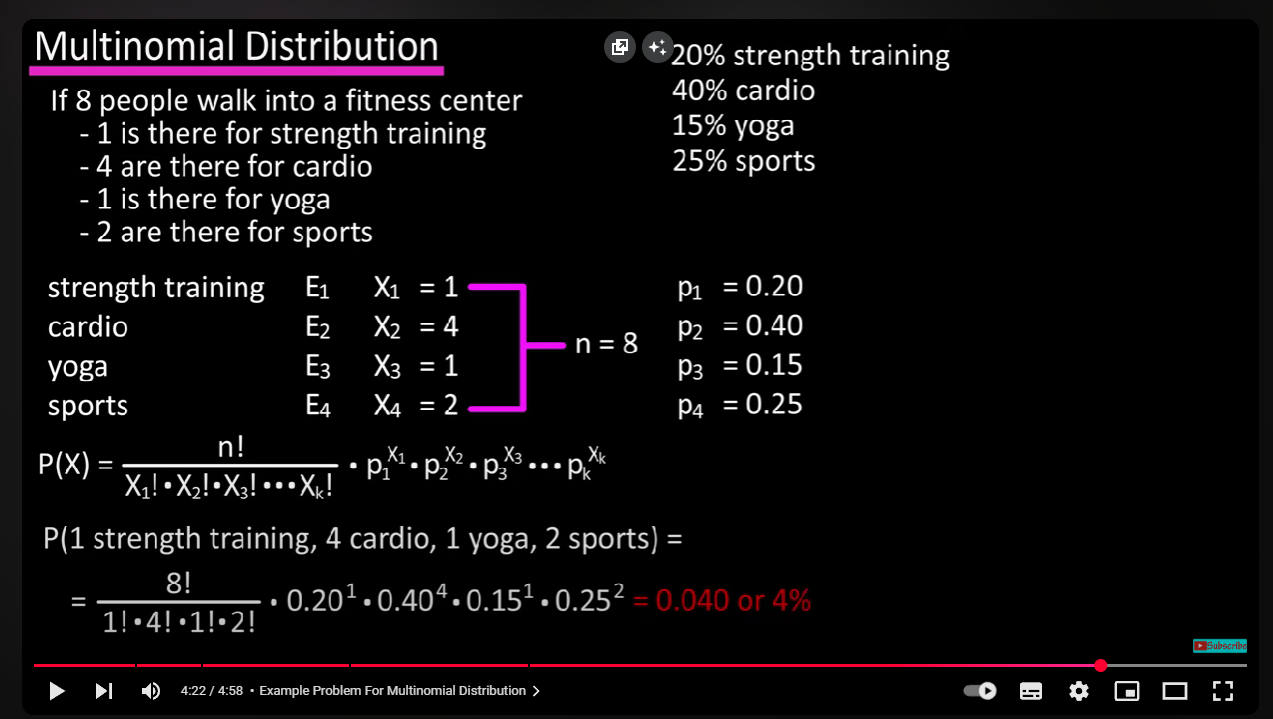
\includegraphics[width=0.6\textwidth]{lawmutinominal.png} % Ajustez le chemin et la taille
		\caption{Illustration de la loi multinomiale.}
		\label{fig:multinomial}
	\end{figure}
	
	\begin{figure}[h!]
		\centering
		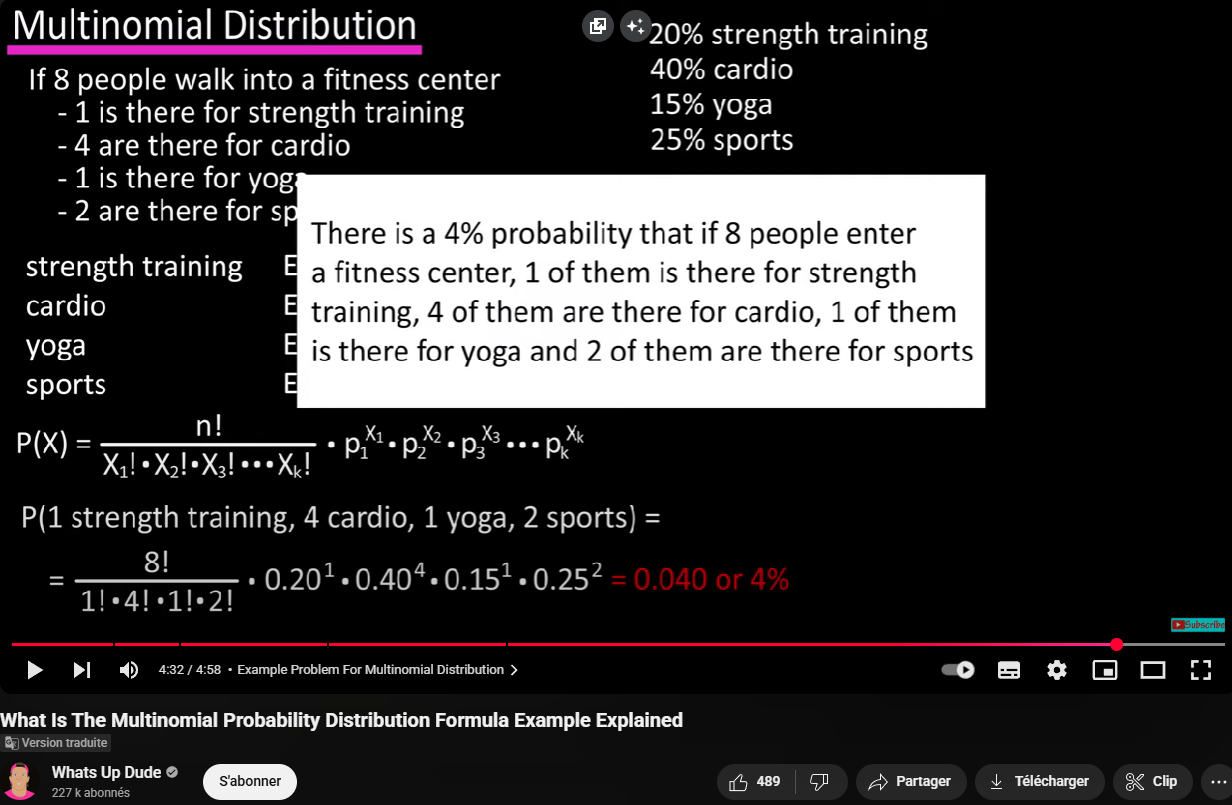
\includegraphics[width=0.6\textwidth]{conclusion.png} % Image nommée 'conclusion'
		\caption{Illustration complémentaire.} % Modifiez la légende si besoin
		\label{fig:conclusion_img}
	\end{figure}
	
	Vidéo (Anglais) : The Binomial Distribution and the Multinomial Distribution \url{https://www.youtube.com/watch?v=UXB9eeMZfwo}
	\\
	\\
	\subsubsection{Gradient} % Correspond au point 9
	Comment calculer le gradient d'une fonction : \url{https://www.youtube.com/watch?v=JiM2iR8gN4M}
	
	\subsubsection{Newton-Raphson} % Correspond au point 10
	Newton-Raphson Formula And Derivation | Part 1 of 2 : \url{https://www.youtube.com/watch?v=YSl37OYMLFw}
	
	
	\section{Applications et résultats} % Correspond au point 6
	L’algorithme est appliqué à la modélisation de données d’accidents de la route, pour estimer l’effet moyen d’une mesure de sécurité et les risques associés.
	Les simulations montrent une meilleure performance par rapport aux méthodes classiques, en particulier en termes de vitesse de convergence et de robustesse aux choix initiaux.
	% Vous pouvez ajouter plus de détails ici si vous les avez.
	
	\section{Discussion} % Votre structure demandait une section Discussion
	% Vous devrez ajouter votre propre analyse ici.
	Analysez les avantages, limites et perspectives de l’approche.
	
	\section{Conclusion} % Correspond à "## Conclusion"
	L’article propose une alternative efficace et explicite aux méthodes classiques d’estimation sous contraintes, en tirant parti du complément de Schur et d’une démarche cyclique. Cette approche est particulièrement adaptée aux problèmes de grande dimension et à contraintes complexes, comme illustré dans le domaine de la sécurité routière.
	
	Pour toute question sur une notion spécifique, consulte les liens ci-dessus pour des explications détaillées.
	
	\section{Références} % Correspond à "## Références citées dans le document"
	\begin{itemize}
		\item Méthode du maximum de vraisemblance : [1–3] dans le document (références internes à l’article)
		\item Revue complète des méthodes d’optimisation classiques
		\item [5–8] Description de l’algorithme BFGS
		\item Méthode de Nelder–Mead
		\item [10–12] Adaptations des méthodes classiques au maximum de vraisemblance sous contraintes
		\item [13], algorithmes MM (Minorization–Maximization)
		\item Travaux antérieurs des auteurs sur la résolution par systèmes non linéaires
		\item [17–19] Propriétés du complément de Schur
	\end{itemize}
	% Formatez ceci en BibTeX ou manuellement selon vos besoins.
	
	\section{Annexes} % Pour "Liens pour approfondir" et "Questions liées"
	
	\subsection{Liens pour approfondir les notions} % Correspond au tableau Markdown
	\begin{itemize}
		\item \textbf{Maximum de vraisemblance :} \url{https://fr.wikipedia.org/wiki/Maximum_de_vraisemblance}
		\item \textbf{Complément de Schur :} \url{https://fr.wikipedia.org/wiki/Compl%C3%A9ment_de_Schur}
		\item \textbf{Optimisation sous contraintes :} \url{https://fr.wikipedia.org/wiki/Programmation_math%C3%A9matique}
		\item \textbf{Méthode de Newton-Raphson :} \url{https://fr.wikipedia.org/wiki/M%C3%A9thode_de_Newton}
		\item \textbf{Méthode BFGS :} \url{https://en.wikipedia.org/wiki/Broyden%E2%80%93Fletcher%E2%80%93Goldfarb%E2%80%93Shanno_algorithm}
		\item \textbf{Méthode Nelder-Mead :} \url{https://fr.wikipedia.org/wiki/M%C3%A9thode_de_Nelder-Mead}
		\item \textbf{Algorithmes MM :} \url{https://en.wikipedia.org/wiki/Expectation%E2%80%93maximization_algorithm#Relation_to_MM_algorithms}
	\end{itemize}
	
	\subsection{Questions liées} % Correspond à "## Questions liées"
	\begin{itemize}
		\item Quelles sont les notions clés du complément de Schur et leurs applications ?
		\item Où puis-je trouver des ressources détaillées sur la décomposition en blocs de l'opérateur A ?
		\item Comment le complément de Schur facilite la résolution de systèmes linéaires complexes ?
		\item Quelles références académiques ou liens pour approfondir la théorie du complément de Schur ?
		\item Existe-t-il des exemples concrets ou études de cas illustrant l'utilisation du complément de Schur ?
	\end{itemize}
	
\end{document}